\documentclass[12pt]{article}

\usepackage{sbc-template}
\usepackage{graphicx,url}
\usepackage[utf8]{inputenc}
\usepackage[brazil]{babel}
\usepackage{subcaption}

     
\sloppy

\title{Análise de Escalabilidade Horizontal em um~\emph{cluster}  Hbase}

\author{Bruno Santos de Lima, Cedryk Augusto dos Santos, Ronaldo Celso Messias Correia }


\address{Faculdade de Ciências e Tecnologia -- Universidade Estadual Paulista (UNESP)\\
  Presidente Prudente -- SP -- Brazil
  \email{bruno.s.lima@unesp.br,cedrykaugusto@gmail.com,ronaldo.correia@unesp.br}
}

\begin{document} 

\maketitle

%Resumo maximo 10 linhas.
%Se o artigo estiver em português o abstract deve estar localizado antes do resumo.

\begin{abstract}
NoSQL databases facilitate horizontal scheduling, allowing the distribution of resources from the addition of nodes. In this context, this work evaluates the horizontal scaling potential of a HBASE database cluster through a benchmarking of several scenarios to verify the efficiency and availability of applications regardless of the size of the storage demand and operations, as of the addition we. The results show that scalability is more evident, except for ~\emph{scan} operations, in sets in the proportion of 100,000 and 1,000,000 records of 1KB each, in increasing the number of nodes from 1 to 2 and of 2 to 3. In the search operations, there is no improvement in the performance from the insertion of nodes, due to the linear search method.
\end{abstract}
     
\begin{resumo} 
%Com o surgimento do Big Data, identificou-se cenários onde a complexidade lógica existente na modelagem relacional não é necessária e novas soluções com características diferentes foram propostas, denominadas bancos de dados NoSQL. Os bancos de dados NoSQL tem como principal característica o escalonamento horizontal, em que os recursos de um sistema computacional aumenta com a adição de novos nós em um ambiente distribuído (cluster), em vez de substituição por um hardware mais potente. Diante disso, este trabalho avalia o potencial do escalonamento horizontal de um~\emph{cluster}  executando o banco de dados NoSQL Hbase, realizando um benchmarking sobre diversos cenários, analisando se com o uso deste paradigma as aplicações podem continuar eficientes e disponíveis independente do tamanho da demanda de armazenamento e de consultas, quando há a adição novos nós no sistema. Os experimentos mostraram que a escalabilidade horizontal existe e é mais evidente, exceto para operações~\emph{scan} (busca), em conjuntos de dados maiores que no contexto dessa pesquisa foram de que neste trabalho foram 100.000 e 1.000.000 de registros de 1KB de tamanho cada e ao se aumentar o número de nós de 1 para 2 e, de 2 para 3 nós. No caso dos testes que executaram operações de busca, não há melhora no desempenho a medida que nós são adicionados ao sistema, devido ao método de busca implementado pelo Hbase ser linear
Os bancos de dados NoSQL facilitam escalonamento horizontal, permitindo a distribuição de recursos a partir da adição de nós. Nesse contexto, este trabalho avalia o potencial do escalonamento horizontal de um~\emph{cluster}  do banco de dados Hbase, através de um benchmarking sobre diversos cenários, de modo a verificar a eficiência e disponibilidade de aplicações independentemente do tamanho da demanda de armazenamento e operações, a patir da adição nós. Os resultados demonstram que a escalabilidade é mais evidente, exceto para operações~\emph{scan}, em conjuntos na proporção de 100.000 e 1.000.000 de registros de 1KB cada, no aumento do número de nós de 1 para 2 e, de 2 para 3. Nas operações de busca, não há melhora no desempenho a partir da inserção de nós, devido ao método de busca linear.
\end{resumo}


\section{Introdução}
\label{sec:introducao}

%Um dos grandes desafios computacionais é o armazenamento e a recuperação de dados de forma eficiente, para que possam ser acessados rapidamente e que estejam sempre disponíveis a quem os requisite. 
Um dos grandes desafios computacionais consiste no armazenamento, recuperação e disponibilidade de dados de modo eficiente.
Durante muitos anos, a solução para a maioria dos problemas dessa área foram os sistemas gerenciadores de banco de dados relacionais (SGBDR), que garantem as propriedades de atomicidade, de consistência, de isolamento e de durabilidade (ACID). 
%Porém, a maioria dos SGBDR’s não atendem mais de forma satisfatória às necessidades de certos cenários identificados com surgimento do~\emph{Big Data}[Brito 2010].
Contudo, os SGBDR’s não satisfazem as necessidades de sistemas no âmbito de~\emph{Big Data}~\cite{brito2010bancos}.

%O conceito de Big Data refere-se ao grande volume de dados gerados em diversos domínios de aplicação, como: a Web, dispositivos móveis, sensores, motores de busca e principalmente nas redes sociais; volume este que está na ordem de 1 Zettabyte/dia [Index 2017] e, as tecnologias criadas para a manipulação desses dados garantindo escalabilidade, confiabilidade e tolerância a falhas [Han et al. 2011]. 
O conceito de Big Data refere-se ao grande volume de dados gerados em diversos domínios de aplicação~\cite{index2013zettabyte,han2011survey}.
%A partir deste conceito, identificou-se que a tecnologia relacional possui grande fragilidade no tratamento de dados classificados como semiestruturados e não estruturados (vídeos, áudios e posts em redes sociais), por exemplo, a dificuldade em acomodá-los no modelo relacional e a dificuldade de implementação distribuída (escalabilidade horizontal) de modo a continuar atendendo às propriedades ACID. A complexidade lógica existente na modelagem relacional somada ao volume exagerado de dados mostrou-se um problema pois pode propiciar deadlocks, problemas de concorrência e lentidão na leitura e escrita dos dados [Han et al. 2011] [Brito 2010].
A partir desse conceito, identificou-se que a tecnologia relacional possui grande fragilidade no tratamento de dados classificados como semiestruturados e não estruturados e dificuldade de implementação distribuída, de modo a atender as propriedades ACID. 
A complexidade lógica existente na modelagem relacional somada ao volume exagerado de dados mostrou-se um problema pois pode propiciar deadlocks, problemas de concorrência e lentidão na leitura e escrita dos dados~\cite{han2011survey,brito2010bancos}.
%Como alternativa para esses cenários, surgiram os bancos de dados denominados NoSQL. Esse termo refere-se aos bancos de dados que não utilizam linguagem SQL para consulta de dados (Not Only SQL), não utilizam do modelo relacional e que em maioria são distribuídos. Tal tecnologia trabalha de forma mais eficiente com grande volume de dados, possibilitando escalar horizontalmente operações por diversos servidores, replicar e distribuir esses dados, adicionar dinamicamente novos atributos aos registros, entre outras. Embora o conceito das ferramentas não relacionais tenha sido apresentado com caráter comparativo, o objetivo destas não é substituir o modelo relacional em todas as situações, apenas nos casos em que é possível adotar uma maior flexibilidade de estruturação e assim, escalonar horizontalmente o sistema de forma eficiente [Brito 2010].
Como alternativa surgiram os bancos de dados denominados NoSQL, os quais atuam de modo mais eficiente com grande volume de dados, possibilitando a distribuição e replicação de dados e operações, além de maior flexibilidade dos dados. 
%Embora o conceito das ferramentas não-relacionais tenha sido apresentado com caráter comparativo, o objetivo destas não é substituir o modelo relacional em todas as situações, apenas nos casos em que é possível adotar uma maior flexibilidade de estruturação e assim, escalonar horizontalmente o sistema de forma eficiente [Brito 2010].

%No contexto deste trabalho, foi utilizado o ambiente de desenvolvimento estabelecido pelo framework open-source Hadoop, desenvolvido pela~\emph{Apache Foundation}, que reúne várias ferramentas de manipulação Big Data em um ponto central, envolvendo bancos de dados NoSQL (Hbase), um sistema de arquivos distribuídos denominado Hadoop Distributed File System (HDFS) e um modelo de programação para suportar computações paralelas em grandes coleções de dados em~\emph{cluster} s de computadores chamado MapReduce [Apache Hadoop 2016].
No contexto deste trabalho, foi utilizado o ambiente de desenvolvimento Hadoop, desenvolvido pela~\emph{Apache Foundation} que reúne ferramentas de manipulação~\emph{Big Data}, envolvendo o banco de dados Hbase, o sistema de arquivos distribuídos~\emph{Hadoop Distributed File System} (HDFS) e o modelo de suporte a programação paralela em grandes coleções de dados chamado MapReduce~\cite{hadoophbase}.

%O banco de dados Hbase, utilizado neste trabalho, permite o processamento distribuído por meio de~\emph{cluster} s. Funciona sobre o HDFS, proporcionando à ferramenta capacidades parecidas ao BigTable /citechang2008bigtable e alta tolerância a falhas ao armazenar grandes quantidades de dados esparsos [Hadoop Hbase 2016].
O banco de dados Hbase permite o processamento distribuído por meio de~\emph{cluster} s, atuando sobre o HDFS de modo a agregar à ferramenta capacidades semelhantes ao BigTable~\cite{chang2008bigtable} e alta tolerância a falhas ao armazenar grandes quantidades de dados esparsos~\cite{hadoophbase}.

%O objetivo deste trabalho é verificar o potencial desse novo paradigma de armazenamento e recuperação de dados que utiliza de computação distribuída para criar um cenário onde aplicações e serviços continuem eficientes e disponíveis independente do tamanho da demanda de armazenamento e de consultas, apenas pela adição de novos nós ao ambiente distribuído. Dessa forma, foi avaliada a escalabilidade horizontal do banco de dados Hbase por meio de benchmarking com operações~\emph{read},~\emph{write},~\emph{scan} e~\emph{read} modifywrite, utilizando o framework Yahoo! Cloud Serving Benchmark (YCSB) a medida em que novos nós são adicionados ao sistema e o tamanho do conjunto de dados é aumentado.
O objetivo deste trabalho consiste em verificar o potencial desse novo paradigma de armazenamento e recuperação de dados utilizando computação distribuída, de modo a criar um cenário, em que aplicações e serviços se mantenham eficientes e disponíveis independentemente do tamanho da demanda de armazenamento e consultas, somente através da adição de novos nós ao ambiente distribuído. 
Desse modo, foi avaliada a escalabilidade horizontal do banco de dados Hbase, através da execução de um~\emph{benchmarking} com operações~\emph{read},~\emph{write},~\emph{scan} e~\emph{read-modify-write} utilizando o framework~\emph{Yahoo! Cloud Serving Benchmark} (YCSB) a partir da inserção de novos nós ao sistema e o crescimento do conjunto de dados.

O restante do trabalho está organizando do seguinte modo: na Seção~\ref{section:fundamentacao} são apresentados conceitos de escalabilidade em banco de dados e as ferramentas utilizadas. Em seguida, a Seção~\ref{section:metodologia} apresenta os cenários de testes utilizados, enquanto a Seção~\ref{section:resultados} exibe a análise quanto aos resultados obtidos. Por fim, a Seção~\ref{sec:finais} apresenta as considerações finais deste trabalho.


\section{Fundamentação Teórica}
\label{section:fundamentacao}

\subsection{Escalabilidade em Banco de Dados}
\label{sec:escalabilidade}

%Segundo [Elmasri and Navathe 2015], a escalabilidade é a capacidade de expandir os recursos de um sistema (capacidade de armazenamento e de processamento). Aplicando ao contexto deste artigo podemos dizer que um banco de dados escalável possui a habilidade de manipular/processar quantidades de dados cada vez maiores e, garantir a disponibi- lidade do sistema. Porém, existem duas abordagens para expandir um sistema as quais estão representadas na Figura 1.
Escalabilidade é a capacidade de expandir os recursos de um sistema (capacidade de armazenamento e de processamento)~\cite{elmasri2010fundamentals}. 
No contexto de banco de dados, um banco de dados escalável tem a capacidade de manipular quantidades de dados cada vez maiores e garantir a disponibilidade do sistema. 
Existem dois tipos de escalabilidade:~\emph{escalabilidade vertical} e~\emph{escalabilidade horizontal}.

A~\emph{escalabilidade vertical}, tradicionalmente usado pelos bancos de dados relacionais, consiste em adicionar mais recursos (CPU / Memória RAM / Disco Rígido) ao servidor. 
Essa é caracterizada pelo menor consumo de energia, menor custo com arrefecimento e geralmente mais fácil implementação. Por outro lado, possui maior custo e possibilidade de interrupção do serviço sendo por falha (centralização do sistema) ou limitação das possibilidades de~\emph{upgrade} da máquina atual, requerindo a transferência do sistema para outro servidor~\cite{hwang2014scale}.

Em contraponto, na~\emph{escalabilidade horizontal}, os recursos não são centralizados em um servidor, mas sim distribuídos em diversos servidores. 
Geralmente, os servidores incluídos consistem em máquinas simples, com o propósito de redução de custos.  
Adicionalmente, há garantia de recuperação a falhas, em que a paralisação de uma máquina não causa a interrupção do sistema, devido a presença de redundância de dados e processos nos demais nós.
Essa arquitetura é muito semelhante em diversos banco de dados NoSQL~\cite{hwang2014scale}, assim como no HBase, utilizado neste trabalho.

\subsection{Apache Hadoop}
\label{section:ferramentas}

%A biblioteca de softwares Apache Hadoop é um conjunto de aplicações (framework) que permite o processamento distribuído de um grande volume de dados em~\emph{cluster} s por meio de um modelo de programação simples conhecido como MapReduce, o qual é projetado para escalar horizontalmente o processamento, oferecer alta disponibilidade e recuperação de falhas [Apache Hadoop 2016].
A biblioteca de softwares Apache Hadoop consiste em um conjunto de aplicações (\textit{framework}) para processamento distribuído de grande volume de dados em~\emph{cluster} s. Esse utiliza o modelo de programação simples MapReduce, projetado para escalonamento horizontal, oferecendo alta disponibilidade e recuperação de falhas~\cite{hadoophbase}.
Existem diversas versões adaptadas da ferramenta, com funcionalidades direcionadas a aplicações específicas, muitas vezes desenvolvidas por empresas~\cite{goldman2012apache}.


Um~\emph{cluster}  Hadoop opera sob a arquitetura mestre/escravo, como apresentado na Figura~\ref{figure:hadoop}. 
Em uma aplicação típica existem cinco processos envolvidos. 
O~\emph{NameNode},~\emph{SecondaryNameNode} e o~\emph{JobTraker} são processos únicos para toda a aplicação, em que o~\emph{NameNode} e~\emph{JobTracker} são executados pelo nó-mestre, enquanto~\emph{SecondaryNameNode} pelo nó-mestre ``reserva'' , em caso de falha. 
O~\emph{DataNode} e~\emph{TaskTraker} atuam como processos escravos de multiplas instâncias. 
Por fim, os processos~\emph{NameNode},~\emph{SecondaryNameNode} e~\emph{DataNode} fazem parte da execução do HDFS, enquanto~\emph{JobTraker} e~\emph{TaskTraker} parte da execução MapReduce~\cite{goldman2012apache}.

\begin{figure}[!ht]
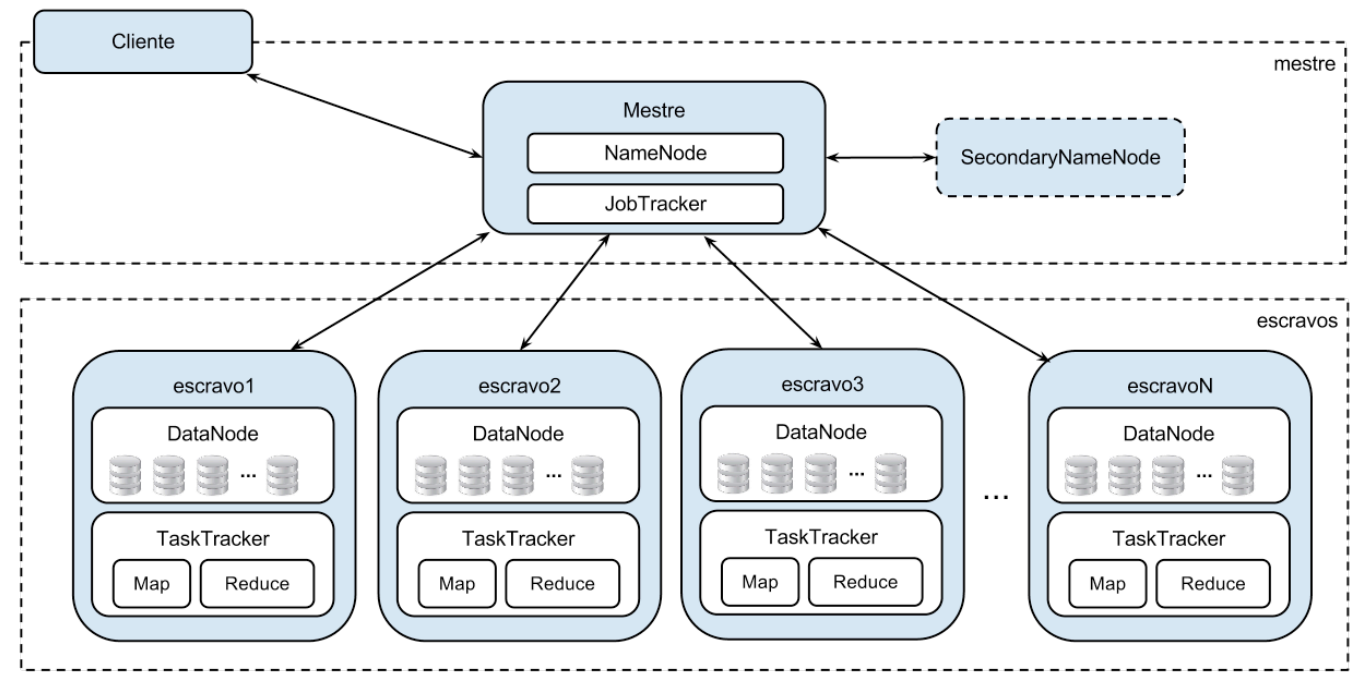
\includegraphics[width=\textwidth]{images/hadoop.png}
\caption{Representação da estrutura dos processos do Hadoop~\cite{goldman2012apache}.}
\label{figure:hadoop}
\end{figure}

\subsection{HDFS}

O HDFS consiste em um sistema de arquivos distribuídos projetado para ser tolerante a falhas, voltado para~\emph{hardwares} de baixo custo que com suporte à máquina virtual Java e aplicações com grande volume de dados. 
Assim como um sistema de arquivos, o HDFS fornece operações de armazenamento, organização, nomeação, atribuição de permissões de acesso, compartilhamento e recuperação de forma transparente ao usuário, porém, o diferencial está no armazamento dos arquivos, os quais compartilhados por máquinas remotas ligadas em rede.

O processo~\emph{NameNode} tem responsabilidade pela abertura, fechamento ou renomeação de arquivos e diretórios; realizar o controle de acesso dos arquivos, armazenar metadados, coordenar a fragmentação dos arquivos em blocos, assim como a distribuição dos mesmos dentro dos processos~\emph{DataNodes}. 
Para os processos~\emph{DataNode} cabe a tarefa de armazenar os dados, responder as solicitações de leitura e escrita dos clientes e aplicações; e criar, remover ou replicar blocos sob orientação do~\emph{NameNode}. 
Além de armazenar, os~\emph{DataNode} precisam se comunicar constantemente com o~\emph{NameNode} para manter o mapeamento dos blocos atualizado e livre de falhas~\cite{hadoophdfs}.

\subsection{HBase}

O Hbase é um banco de dados não-relacional, distribuído, tolerante a falhas, de código aberto e altamente escalável. Tem como foco aplicações que necessitam de leitura e escrita de acesso aleatório com tempo constante em grandes volumes de dados~\cite{hadoophbase}.
O projeto foi inspirado no BigTable da Google, em que ambos utilizam o modelo de dados orientado a colunas. 
Esse não possui nenhuma linguagem de consulta estruturada, porém fornece uma API Java que possibilita realizar operações básicas como~\emph{put},~\emph{get},~\emph{update} e~\emph{delete}. 
Possibilita também o uso da função~\emph{scan}, para selecionar quais as colunas a serem retornadas ou o número de versões de cada célula. Consultas mais complexas ficam a cargo de jobs do MapReduce~\cite{cunha2015column}.

%Geralmente ocorre uma confusão conceitual sobre a diferença entre o HBase e o HDFS. O HDFS é um sistema de arquivos que não fornece pesquisa de registros individuais, enquanto o HBase é executado em cima do HDFS e utiliza indexação para recuperar rapidamente os dados armazenados no HDFS [Hadoop Hbase 2016].

%O HBase utiliza estrutura de mestre/escravo que, na parte mestre do sistema existe o servidor HMaster e o ZooKeeper onde o primeiro controla os servidores escravos chamados~\emph{region servers} (responsáveis pela leitura e escrita), enquanto o segundo é responsável por monitorar e manter o~\emph{cluster}  ativo. 

%Todos os dados do HBase são armazenados como arquivos do HDFS. Dessa forma, os~\emph{region servers} são dispostos nos nós que executam os processos DataNode do HDFS provendo localidade nos dados que transitam de um para o outro[McDonald 2015].

%Figura 3

\section{Yahoo! Cloud Serving Benchmark}

O YCSB (\emph{Yahoo! Cloud Serving Benchmark}) é um framework de código-aberto para apoio a~\emph{benchmarking} de diferentes bancos de dados distribuídos, a qual permite a extensão para banco de dados não implementados previamente~\cite{cooper2010benchmarking}. 
O YCSB possibilita a avaliação de duas ``camadas'' de benchmark: performance e escalabilidade. 
Em performance, mede-se a latência (tempo de execução) das requisições enviadas ao banco e, em escalabilidade é medido o impacto na performance quando o número de servidores do sistema cresce~\cite{cooper2010benchmarking}.

É composto por um conjunto de~\emph{workloads} denominado~\emph{Core Package} e uma aplicação chamada YCSB Client. 
As~\emph{workloads} consistem de combinações de operações de leitura e escrita que atuam sobre um conjunto de dados de certo tamanho e distribuição.
Na execução de uma~\emph{workload}, o YCSB Client realiza a interpretação do arquivo descritor, criando o conjunto de dados e submete as requisições ao banco de dados~\cite{cooper2010benchmarking}. 
%O componente que interpreta e executa as~\emph{workloads} (\emph{Workload} executor) pode ser dividido em múltiplas~\emph{threads} aumentando o número de requisições simultâneas que podem ser enviadas. As~\emph{threads} do YCSB Client então se comunicam com a interface do banco de dados, no qual são traduzidos os comandos descritos na~\emph{workload} para a sintaxe do banco [Cooper et al. 2010].
%A execução dos testes : A load phase, onde o conjunto de dados especificado é gerado e inserido e; A transaction phase onde são executadas as operações definidas. Ao final do processo é gerado um relatório com a latência e o desempenho alcançado em termos de operações por segundo das tarefas executadas. A estrutura do YCSB Client é mostrada na Figura 4.
%Utilizou-se do termo~\emph{threads} no contexto deste trabalho para se referir as~\emph{threads} do YCSB Client.

%Figura 4

\section{Trabalhos Relacionados} 
\label{section:relacionados}

Na apresentação do framework YCSB,~\cite{cooper2010benchmarking} aplicaram~\emph{benchmarking} nos banco de dados Cassandra, Hbase, Yahoo!’s PNUTS e o Sharded MySQL para exemplificar seu uso de maneira prática. A partir de testes de performance e escalidade, concluiram que, assim como suposto pelas descrições dos desenvolvedores, Cassandra e Hbase apresentam maior latência para operações~\emph{read} e menor latência para operações~\emph{update} e~\emph{write} em relação ao PNUTS e MySQL, enquanto o PNUTS e Cassandra melhor escalabilidade, em detrimento ao HBase, quando o número de servidores no~\emph{cluster}  aumenta proporcionalmente a carga de trabalho.
%Escalabilidade esta, que daremos maior foco ao decorrer do artigo; Cassandra, Hbase e PNUTS são aptos a crescer elasticamente durante a execução de uma carga de trabalho, porém o PNUTS apresenta uma latência melhor e mais estável para tal.

\cite{jogi2016performance} realizam a comparação MySQL com Cassandra e Hbase quanto a operações~\emph{heavy~\emph{write}}. 
Na condução do teste foi elaborada uma aplicação~\emph{web} REST (\emph{Representacional State Transfer}) para recebimento dos dados e armazenamento no banco de dados. A partir dos resultados, foi possível concluir que o Cassandra apresenta melhor desempenho entre os três bancos quanto a velocidade de escrita, enquanto o Hbase foi duas vezes mais rápido que o MySQL. 
Para~\cite{jogi2016performance}, o comportamento do Cassandra ocorre devido a incorporação de características do Big Table do Google e do DynamoDB.

\cite{swaminathan2016quantitative} realizaram a análise da escalabilidade dos bancos de dados Hbase, Cassandra e MongoDB. Para isso foi utilizado o framework YCSB com diferentes cargas de trabalho e conjunto de trabalho, com o intuito de evidenciar as vantagens e desvantagens de cada ferramenta para um cenário específico com base nas diferenças de design.

Para~\cite{waage2014benchmarking}, a confiabilidade para o armazenamento ``em nuvem'' é um dos pontos chaves para adoção de tecnologias não-relacionais. Desse modo, é proposto que os dados sejam criptografados de modo prévio. Para avaliar o impacto da criptografia, foi realizado um estudo com os bancos de dados Cassandra e Hbase. 
Neste estudo foi utlizado o framework YCSB em que~\emph{workloads} foram aplicadas a dados não-encriptados e encriptados usando o algoritmo~\emph{Advanced Encryption Standard} (AES) com chaves de 128, 192 e 256 bits de comprimento. 
A partir disso, foi relatada uma redução no desempenho médio do~\emph{cluster} , o qual é independente do tamanho da chave de encriptação.

\section{Metodologia}
\label{section:metodologia}

Os testes conduzidos foram executados em um~\emph{cluster}  composto de sete computadores, sendo o nó mestre denominado hpcdmc e os seis nós escravos denominados de n01 a n06, cujas configurações estão descritas abaixo.

Configuração do mestre (hpcdmc):
\begin{itemize}
\item Sistema Operacional Linux CentOS 6.6
\item 2x Processador Intel Xeon E5-2620 2.0GHz 6 núcleos
\item 4x Memória Ram Kingston DDR3 8GB 1333MHz
\item 8x Sata3 de 2TB
\end{itemize}

Configuração dos nós escravos e cliente (n01 a n06):

\begin{itemize}
\item Sistema Operacional Linux CentOS 6.6
\item 2x Processador Intel Xeon E5-2690 2.90GHz 8 núcleos
\item 4x Memória Ram Kingston DDR3 8GB 1600MHz
\item 8x Sata3 de 500GB e 16MB de cahce
\end{itemize}

As versões dos softwares utilizados para a execução dos testes foram escolhidas
por serem as mais atuais e estáveis 1 consultadas no site dos desenvolvedores no início do
trabalho. São elas:

\begin{itemize}
\item Hadoop 2.7.3
\item HBase 1.2.4
\item ZooKeeper 3.4.10
\item YCSB 0.12.0
\end{itemize}

Os testes foram organizados em seis cenários onde, os testes executados nos cinco primeiros cenários analisam a melhor alternativa para a implementação do~\emph{cluster} , ou seja, como serão dispostos os processos cliente, mestre e escravo. 
Nesses foram executados os testes em um ambiente pseudo distribuído, com apenas duas~\emph{workloads}: 100\%~\emph{write} -- 100.000 registros e 100\%~\emph{read} - 100.000 registros, tendo cada registro 1KB e com distribuição uniforme. Cada teste sobre uma~\emph{workload} foi executado 3 vezes para uma dada quantidade de~\emph{threads} do YCSB Client e então foi realizada a média da latência (tempo de execução em milissegundos) e do desempenho médio (operações/segundo) para obter o resultado final do teste.
Nos testes executados no sexto cenário, configurado de acordo com as conclusões obtidas nos testes dos cenários anteriores, é analisada a escalabilidade do HBase em um~\emph{cluster}  totalmente distribuído, sendo esse, o foco principal do trabalho. Cada teste sobre uma~\emph{workload} também foi executado 3 vezes sendo o resultado final a média das saídas.

\subsection{Cenário 1}

No cenário 1 o~\emph{cluster}  é configurado de modo pseudo distribuído, ou seja, os processos são executados como se houvesse uma distribuição entre máquinas em redes, porém estão todos no mesmo nó. Dessa forma, os processos mestre e escravo do Hadoop e HBase, os processos do ZooKeeper e do YCSB Client são executados todos no hpcdmc.
A distribuição dos processos em um~\emph{cluster}  pseudo distribuído é representada pela Figura
5.

\subsection{Cenário 2}

No cenário 2, considerando que a execução de todos os processos mestre e escravo junto com o YCSB Client pode comprometer a quantidade de requisições enviadas ao banco, alocou-se o YCSB em um nó separado para verificar essa hipótese. Dessa forma, os processos meste e escravo do Hadoop e HBase e os processos do ZooKeeper continuaram a ser executados no hpcdmc, mas o processo YCSB Client foi executado no nó n01 conforme é apresentado na Figura 6.

\subsection{Cenário 3}

Dada a limitação do número de~\emph{threads} do YCSB Client que podem ser executadas no n01, pelo número de núcleos do processador, no cenário 3, a execução da~\emph{workload} foi dividida entre nós n01 e n02. Assim, cada nó foi encarregado pela metade dos registros e metade do número de~\emph{threads} do YCSB Client total do teste. Exemplo: na execução da~\emph{workload} 100\%~\emph{read} -- 100.000 registros e 64~\emph{threads}, cada nó gerou 50.000 requisições~\emph{read} com 32~\emph{threads} ativas no YCSB. A saída de cada teste foi a soma do desempenho médio (operações/segundo) e a maior latência (tempo de execução em milissegundos) de ambos. O hpcdmc permaneceu pseudo distribuído conforme é apresentado na Figura 7.

\subsection{Cenário 4}
O cenário 4 se aproxima de uma situação mais adequada quanto a configuração do~\emph{cluster} , onde os processos cliente, mestre e escravo estão completamente distribuíos. O n01 é responsável pelo YCSB Client, o hpcdmc pelos processos mestre do Hadoop, HBase e dos processos do ZooKeeper, enquanto o n02 executou os processos escravos do Hadoop e HBase conforme é apresentado na Figura 8.

\subsection{Cenário 5}
No cenário 5, o objetivo dos testes é analisar se é necessário mais de um servidor gerando
requisições para saturar um~\emph{cluster}  completamente distribuío. Assim, o n01 e n02 dividiram a execução das~\emph{workloads}, o hpcdmc foi responsável pelos processos mestre doHadoop, HBase e os processos do ZooKeeper e o n03 executou os processos escravos do Hadoop e HBase conforme é apresentado na Figura 9.

\subsection{Cenário 6}
Os resultados dos testes realizados nos cenários anteriores apoiam as decisões quanto a estrutura geral do cenário 6 ilustrado na Figura 10. Foram executadas as~\emph{workloads}:~\emph{write},~\emph{read} e~\emph{scan}, variando entre 1.000, 10.000, 100.000 e 1.000.000 registros com tamanho igual a 1KB e com distribuição uniforme, variando o número de escravos de 1 a 5 e o número de~\emph{threads} do YCSB Client fixo.

\section{Resultados e Discussões}
\label{section:resultados}

\subsection{Resultados dos Cenários de 1 a 5}

Nos resultados obtidos nos cenários 1 e 2 indicam um crescimento no desempenho médio do~\emph{cluster} nas execuções com até 64~\emph{threads}, como ilustram as Figuras~\ref{figura11} e~\ref{figura13}.
No cenário 1, entre 1 e 64~\emph{threads} ocorreu um aumento de aproximadamente 90\% no desempenho médio e, enquanto no cenário 2 ocorreu, para a mesma quantidade de~\emph{threads}, um aumento de aproximadamente 93\%.

\begin{figure*}
    \centering
    \begin{subfigure}[b]{0.49\textwidth}
        \centering
        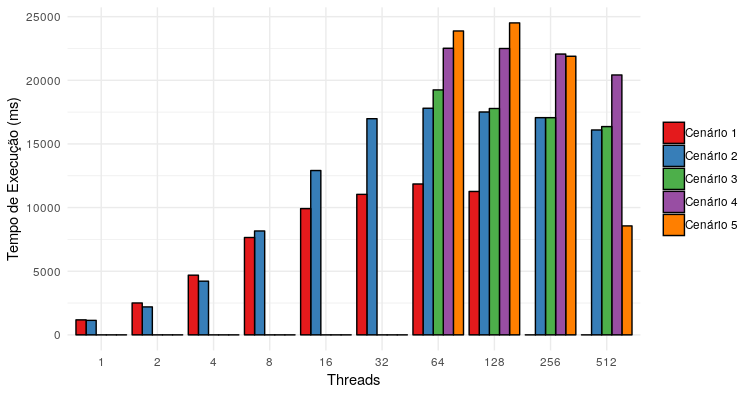
\includegraphics[width=\textwidth]{images/figura11}
        \caption{Desempenho médio.}
        \label{figura11}
    \end{subfigure}
        \hfill
    \begin{subfigure}[b]{0.49\textwidth}  
        \centering 
        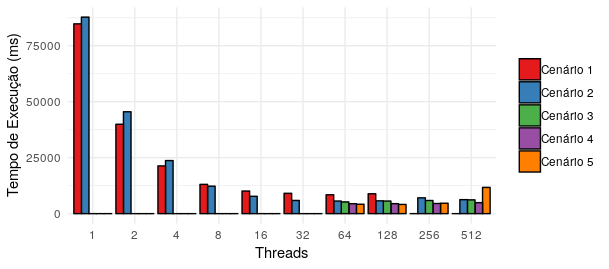
\includegraphics[width=\textwidth]{images/figura12}
        \caption{Latência.}%
        \label{figura12}
    \end{subfigure}
    \caption{\emph{Workload} 100\%~\emph{write} -- 100.000 registros nos cenários de 1 a 5.}
\end{figure*}

Na instanciação de mais de 64~\emph{threads}, no cenário 1 onbserva-se queda no desempenho médio de aproximadamente 5\% nos testes com 128~\emph{threads} e, no cenário 2, também quedas nas execuções de 128, 256 e 512~\emph{threads}, sendo a mais expressiva de aproximadamente 10\% nas execuções com 256~\emph{threads}. Ambas as porcentagens foram calculadas comparando os resultados às execuções com 64~\emph{threads}.

Da mesma forma, observa-se queda na latência nos testes dos cenários 1 e 2 até as execuções com 64~\emph{threads}, apresentado nas Figuras~\ref{figura12} e~\ref{figura14}. 
Dado a medida que o desempenho médio aumenta, ou seja, o~\emph{cluster} executa mais operações por segundo, o tempo de execução do teste diminui. 
Para o cenário 1, a queda da latência entre as execuções com 1 e 64~\emph{threads} foi de aproximadamente 90\% e, para o cenário 2 de aproximadamente 93\%.

Constata-se que o desempenho máximo do~\emph{cluster}  foi obtido para os dois cenários nas execuções do YCSB Client com 64~\emph{threads} e, a partir do cenário 3 foram executados apenas os testes de 64 a 512~\emph{threads}, de modo a observar se esses resultados foram ótimos locais ou globais. 
Os testes do cenário 1, para 256 e 512~\emph{threads} não puderam ser executados por estouro da pilha de memória do nó hpcdmc ao executar o YCSB Client ja que, além do YCSB Client o nó hpcdmc também estava executando os processos mestre e escravo do Hbase e Hadoop e os processos do ZooKeeper.

A análise dos resultados obtidos pela execução testes com a~\emph{workload} 100\%~\emph{write} -- 100.000 registros, mostrou que o melhor desempenho médio foi alcançado pelo cenário 5 para as execuções com 64 e 128~\emph{threads}, sendo maior que os resultados dos cenários 4, 3, 2 e 1 aproximadamente 5,7\%, 19,4\%, 25,4\% e 50,3\% nas execuções com 64 threads e, 8,2\%, 27,4\%, 28,6\% e 54\% nas execuções com 128~\emph{threads}, respectivamente.
Para as execuções com 256 e 512~\emph{threads} o melhor desempenho médio foi obtido pelo cenário 4 sendo maior que os cenários 5, 3 e 2 aproximadamente 0,8\%, 22,6\% e 35,6\% nas execuções com 256~\emph{threads} e, 58\%, 19,9\% e 21,2\% nas execuções com 512~\emph{threads}respectivamente.

O cenário 5 apresentou esse desempenho pois o~\emph{cluster} foi completamente distribuído, então os processos mestres e escravo do Hbase e Hadoop, os processos do ZooKeeper e YCSB não concorreram por recursos de uma mesma máquina uns com os outros.
O mesmo ocorreu no cenário 4, mas a divisão da execução das~\emph{workloads} entre o n01 e n02 apresentou uma pequena melhora no cenário 5 no desempenho do~\emph{cluster}  executando o YCSB com 64 e 128~\emph{threads}, já nas execuções com 256 e 512~\emph{threads} tal divisão sobrecarregou demais o n03 fazendo com que o desempenho médio diminuísse e a latência aumentasse, tornando os resultados dos testes do cenário 4 melhores.

A partir dos testes da~\emph{workload} 100\%~\emph{write} -- 100.000 registros, pode-se concluir que o cenário 5, para execuções com 64 e 128~\emph{threads} obteve uma execução mais rápida que os testes dos cenários 4, 3, 2 e 1 aproximadamente 5,6\%, 19,7\%, 25,4\% e 50,2\% com 64~\emph{threads} e, 7,8\%, 27\%, 28,1\% e 53,7\% com 128~\emph{threads} respectivamente. 
Enquanto que para as execuções com 256 e 512~\emph{threads} o cenário 4 teve uma execução mais rápida que os testes dos cenários 5, 3 e 2 aproximadamente 2,4\%, 22,8\% e 35,8\% com 256 threads e, 95,8\%, 20,3\% e 21,5\% com 512~\emph{threads}. 
Os resultados são apresentados na Figura~\ref{figura12}.

Analisando os resultados dos testes da~\emph{workload} 100\%~\emph{read} -- 100.000 registros, para todos os números de~\emph{threads} o cenário 5 obteve o melhor desempenho médio sendo maior que os resultados dos testes dos cenários 4, 3, 2 e 1 aproximadamente 26,8\%, 22,2\%, 48,3\% e 62,6\% nas execuções com 64~\emph{threads} e, 26,9\%, 44,3\%, 45,7\% e 64,4\% nas execuções com 128~\emph{threads} respectivamente. 
E maior que os resultados dos testes dos cenários 4, 3 e 2 aproximadamente 28,4\%, 23\% e 50,4\% nas execuções com 256~\emph{threads} e, 26,5\%, 18,2\% e 47,3\% nas execuções com 512~\emph{threads} respectivamente.

Para as operações de leitura especificadas na~\emph{workload} 100\%~\emph{read}, a divisão de requisições entre o n01 e n02 não sobrecarregou o n03 para execuções com 256 e 512 threads como nos testes da~\emph{workload} 100\%~\emph{write}, então o cenário 5 obteve os melhores resultados para cada execução entre 64 e 512~\emph{threads}. 
Os testes do cenário 3, que também dividiram as requisições entre o n01 e n02 obtiveram os segundos melhores resultados para cada execução entre 64 e 512~\emph{threads}. 
Portanto para operações de leitura, o~\emph{cluster}  é mais eficiente, considerando o desempenho médio e a latência, se as requisições são realizadas de mais de um cliente. 
Os resultados são ilustrados na Figura~\ref{figura13}.

\begin{figure*}
    \centering
    \begin{subfigure}[b]{0.49\textwidth}   
        \centering 
        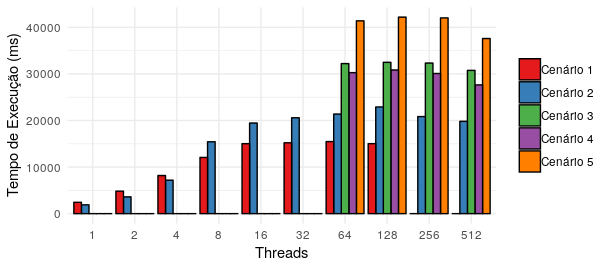
\includegraphics[width=\textwidth]{images/figura13}
        \caption{Desempenho médio.}
        \label{figura13}
    \end{subfigure}
    \begin{subfigure}[b]{0.49\textwidth}   
        \centering 
        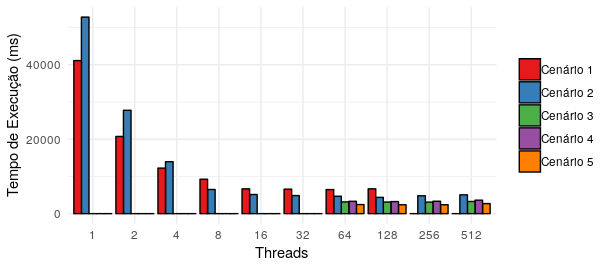
\includegraphics[width=\textwidth]{images/figura14}
        \caption{Latência.}
        \label{figura14}
    \end{subfigure}
    \caption{\emph{Workload} 100\%~\emph{read} -- 100.000 registros nos cenários de 1 a 5.}
\end{figure*}

Na~\emph{workload} 100\%~\emph{read} -- 100.000 registros, cujo os dados são apresentados pela Figura 14, a latência dos testes executados no cenário 5 foi menor que os cenários 4, 3, 2 e 1 aproximadamente 26,2\%, 22,8\%, 47,9\% e 62,3\% nas execuções com 64~\emph{threads} e, 26,6\%, 23,6\%, 45,6\% e 64,3\% nas execuções com 128~\emph{threads} respectivamente. 
E também, menor que os cenários 4, 3 e 2 aproximadamente 27,9\%, 22,8\% e 50\% nas execuções com 256~\emph{threads} e, 25,5\%, 17,3\% e 46.6\% nas execuções com 512~\emph{threads} respectivamente.

Com os resultados observou-se que, para todos os cenários as execuções com 64 e 128~\emph{threads} são as mais altas e a variação referente a um mesmo cenário, considerando essas duas quantidades de~\emph{threads} não são expressivas, sendo de aproximadamente 1\%, para os testes da~\emph{workload} 100\%~\emph{write} e 100\%~\emph{read}, tando para o desempenho médio
quanto para a latência.

O aumento do número de~\emph{threads} além de 128 causou uma queda do desempenho médio nos testes dos cenários 5, 4, 3 e 2 de até 65\%, 9,3\%, 15\% e 9,6\% para os testes da~\emph{workload} 100\%~\emph{write} e, 10,9\%, 10,4\%, 5,3 e 13,5\% para os testes da~\emph{workload} 100\%~\emph{read} respectivamente. 
Comparando então os 5 cenários em que a execução do YCSB Client ocorreu com 64~\emph{threads}, temos que em ambas as~\emph{workloads} 100\%~\emph{write} e 100\%~\emph{read} o cenário 5 obteve o maior desempenho médio do~\emph{cluster}, seguido pelo cenário 4 na~\emph{workload} 100\%~\emph{write} com uma diferença de aproximadamente 5,7\% e, seguido pelos cenários 3 e 4 na~\emph{workload} 100\%~\emph{read} com uma diferença de aproximadamente 22,2\% e 26,8\% respectivamente.

Os testes do cenário 4 obtiveram o segundo maior desempenho médio nos testes da~\emph{workload} 100\%~\emph{write} com uma diferença de menos de 6\% comparado aos resultados do cenário 5, obtiveram o terceiro maior desempenho médio nos testes da~\emph{workload} 100\%~\emph{read} com uma diferença de aproximadamente 6\% comparado com os resultados cenário 3 e, considerando também que ambos os cenários 5 e 3 utilizam 2 nós para a execução do YCSB Client, reduzindo o número de nós disponíveis para os testes de adição de nós, a implementação do~\emph{cluster} para os testes do cenário 6 foi realizada de acordo com o cenário 4 e com 64~\emph{threads} de execução no YCSB Client.


\subsection{Resultados do Cenário 6}

Inicialmente, a respeito do desempenho médio, apresenta na Figura~\ref{figura15}, pode-se notar que a escalabilidade horizontal foi mais evidenciada quando o conjunto de dados foi igual a 1.000.000 de registros, sendo o desempenho do~\emph{cluster} com 5~\emph{region servers} maior do que os testes executados com 4, 3, 2, e 1~\emph{region servers} em aproximadamente 5,1\%, 6,5\%, 17,1\% e 47\% respectivamente. 
Os resultados dos testes em que o conjunto de dados foi igual a 100.000 registros também apresentou certa escalabilidade, sendo o desempenho médio com 5~\emph{region servers} maior do que o desempenho médio dos testes executados com 4, 3, 2, e 1~\emph{region servers} em aproximadamente 9,9\%, 10,4\%, 15,7\% e 43,4\% respectivamente.

\begin{figure*}[!ht]
    \centering
    \begin{subfigure}[b]{0.49\textwidth}
        \centering
        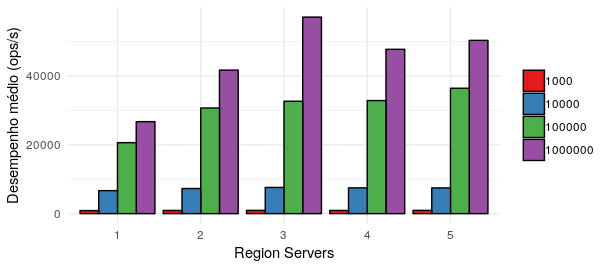
\includegraphics[width=\textwidth]{images/figura15}
        \caption{Desempenho médio.}
        \label{figura15}
    \end{subfigure}
        \hfill
    \begin{subfigure}[b]{0.49\textwidth}  
        \centering 
        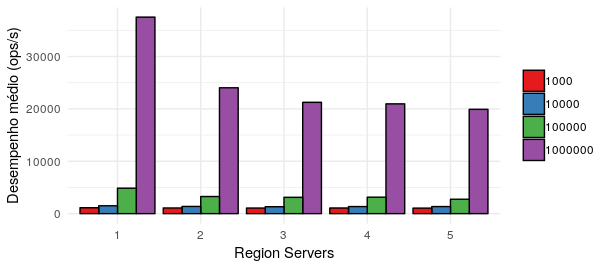
\includegraphics[width=\textwidth]{images/figura16}
        \caption{Latência.}
        \label{figura16}
    \end{subfigure}
    \caption{\emph{Workload} 100\%~\emph{write} variando o tamanho do conjunto de dados e o número de~\emph{region servers} do~\emph{cluster} .}
\end{figure*}

A partir dos resultados dos testes da~\emph{workload} 100\%~\emph{write}, ilustrados na Figura~\ref{figura16}, pode-se observar que os testes que o conjunto de dados foi igual a 1.000.000 de registros obtiveram uma latência menor que os testes com 4, 3, 2 e 1 region server em aproximadamente 5\%, 6,3\%, 17,1\% e 47\% respectivamente. Os resultados dos testes com 100.000 registros, onde a escalabilidade foi menos evidenciada, as latências tiveram poucas alterações comparados os resultados dos testes com 4, 3, 2 e 1 region server, sendo menor em aproximadamente 12,5\%, 11,7\%, 15,9\% e 43,4\% respectivamente.

Os testes em que os conjuntos de dados foram iguais a 1.000 e 10.000 registros não tiveram alterações tão significativas no desempenho médio com a adição de novos nós, sendo a variação mais expressiva para o conjunto de dados de 1.000 registros de aproximadamente 4\% aumentando de 1 para 2~\emph{region servers} e, de aproximadamente 8\% para o conjunto de dados de 10.000 aumentando de 1 para 2 region servers, considerando tanto o desempenho médio quanto a latência como ilustrado pelas Figuras~\ref{figura17} e~\ref{figura18}.

\begin{figure*}[!ht]
    \centering
    \begin{subfigure}[b]{0.49\textwidth}
        \centering
        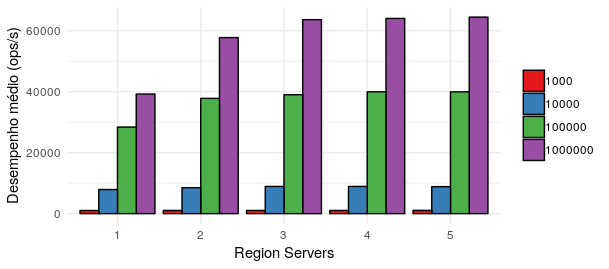
\includegraphics[width=\textwidth]{images/figura17}
        \caption{Desempenho médio.}
        \label{figura17}
    \end{subfigure}
        \hfill
    \begin{subfigure}[b]{0.49\textwidth}  
        \centering 
        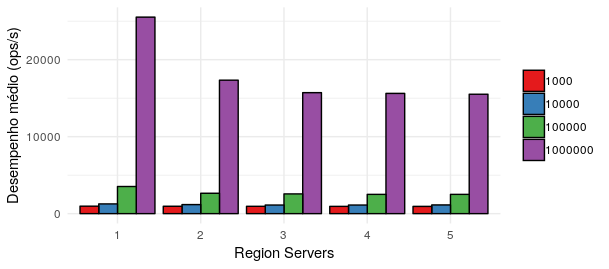
\includegraphics[width=\textwidth]{images/figura18}
        \caption{Latência}%
        \label{figura18}
    \end{subfigure}
    \caption{\emph{Workload} 100\%~\emph{read}  variando o tamanho do conjunto de dados e o número de region servers do~\emph{cluster} .}
\end{figure*}

Para a~\emph{workload} 100\%~\emph{read}, assim como nos resultados acima, nota-se que a escalabilidade horizontal foi mais evidenciada quando o conjunto de dados foi igual a 1.000.000 de registros. 
Porém nas execuções com 5 region servers só existiu alteração significativa no desempenho médio quando comparadas com as execuções com 2 e 1 region servers, sendo maior em aproximadamente 10,4\% e 39,1\% respectivamente. 
Para as execuções com 4 e 3~\emph{region servers} a variação foi de menos de 1,5\% como apresenta a Figura~\ref{figura18}.
Pelos resultados dos testes com 100.000 registros, nota-se o mesmo comportamento, sendo o desempenho médio das execuções com 5~\emph{region servers} maior que os testes com 2 e 1~\emph{region servers} aproximadamente 5,4\% e 29\% respectivamente.
Para as execuções com 4 e 3~\emph{region servers} a variação foi de menos de 2,4\%.

Os testes em que os conjuntos de dados foram iguais a 1.000 e 10.000 registros não tiveram alterações significativas, sendo a variação mais expressiva para o conjunto de dados de 1.000 registros de menos de 1,5\% aumentando de 1 para 2~\emph{region servers} e para o conjunto de 10.000 registros de menos de 7,5\% também aumentando de 1 para 2~\emph{region servers}.

A latência dos testes da~\emph{workload} 100\%~\emph{read} como pode-se analisar nos dados apresentados pela Figura 18, também não apresentou alterações significativas para os testes cujos conjuntos de dados foram iguais 1.000.000 e 100.000 registros quando variados os~\emph{region servers} entre 3 e 5, sendo essa variação de menos de 1,3\% para ambos os con- juntos. Desta forma, os testes executados com 5~\emph{region servers} apresentaram uma latência menor que os testes com 2 e 1~\emph{region servers} em aproximadamente 10,5\% e 40,2\% com 1.000.000 de registros e, em aproximadamente 5,4\% e 29\% com 100.000 registros respectivamente.

Os testes em que os conjuntos de dados foram iguais a 1.000 e 10.000 registros não tiveram alterações significativas no desempenho médio, sendo a variação de 1 para 5 region servers de menos de 3,3\% para o conjunto de 1.000 registros e, de menos de 10,7\% para o conjunto de 10.000 registros.

\begin{figure*}[!ht]
    \centering
    \begin{subfigure}[b]{0.49\textwidth}
        \centering
        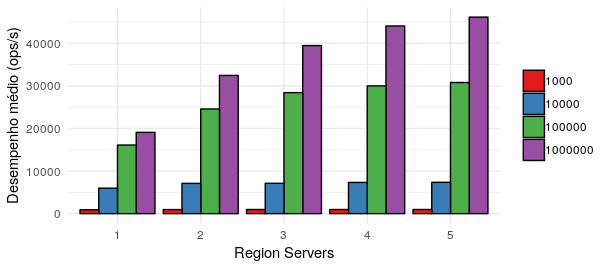
\includegraphics[width=\textwidth]{images/figura19}
        \caption{Desempenho médio.}
        \label{figura19}
    \end{subfigure}
        \hfill
    \begin{subfigure}[b]{0.49\textwidth}  
        \centering 
        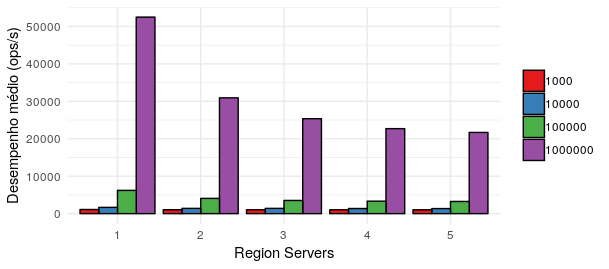
\includegraphics[width=\textwidth]{images/figura20}
        \caption{Latência.}%
        \label{figura20}
    \end{subfigure}
    \caption{\emph{Workload} 100\%~\emph{read/modify/write} variando o tamanho do conjunto de dados e o número de region servers do cluster.}
\end{figure*}

Pela análise dos resultados quanto ao desempenho médio dos testes da~\emph{workload} 100\%~\emph{read}/modify/write, na Figura~\ref{figura19}, observou-se novamente que, a escalabilidade horizontal é mais evidenciada nos cenários onde o conjunto é igual a 1.000.000 de registros, sendo o desempenho médio dos testes com 5~\emph{region servers} maior que os resultados dos testes com 4, 3, 2 e 1~\emph{region servers} aproximadamente 4,5\%, 14,5\%, 29,7\% e 58,6\% respectivamente.
Para os testes onde os conjuntos de dados foram iguais a 100.000 registros obteve-se nas execuções com 5~\emph{region servers} um desempenho médio maior que os testes com 4, 3, 2 e 1 region server de aproximadamente 5,6\%, 7,1\%, 20,1\% e 47,7\% respectivamente.

Os testes onde os conjuntos de dados foram iguais a 1.000 registros não tiveram alterações significativas no desempenho médio, sendo a variação mais expressiva de menos de 6\% aumentando de 1 para 2 region servers. Para o conjunto de 10.000 registro, a variação mais expressiva foi de aproximadamente 18,5\% quando aumentado de 1 para 2 region servers. As demais adições de nós apresentaram uma variação de menos de 4\%.

A Figura 20 apresenta os resultados dos testes da~\emph{workload} 100\%~\emph{read/modify/write} quanto a latência. Novamente, o comportamento da latência acompanha o comportamento do desempenho médio de maneira inversamente proporcional e portanto, os testes com 1.000.000 de registros e 5~\emph{region servers} obtiveram uma latência menor que os testes com 4, 3, 2 e 1~\emph{region servers} em aproximadamente 4,4\%, 14,4\%, 29,9\% e 58,7\% respectivamente. 
Do mesmo modo, os testes com 100.000 registros e 5 region servers obtiveram uma latência menor que os testes com 4, 3, 2 e 1 region servers em aproximadamente 2,6\%, 7,7\%, 20,1\% e 47,9\% respectivamente.

Os testes da~\emph{workload} 100\%~\emph{read/modify/write} em que os conjuntos de dados foram iguais a 1.000 e 10.000 registros não tiveram alterações significativas na latência, seguindo a mesma porcentagem calculada nos testes de desempenho médio.

Os resultados dos testes da~\emph{workload} 100\%~\emph{scan} referentes ao desempenho médio e latência são apresentados nas Figuras 21 e 22. 
Exceto nos testes cujos conjuntos de dados foram iguais a 1.000 registros, não houveram alterações significativas no desempenho médio do~\emph{cluster}  sendo a variação mais expressiva de todos os conjuntos menor que 1,4\%. 
Portanto também não houve alteração significativa na latência em nenhum testes executados.

Para os testes cujo o conjunto de dados foi igual a 1.000 registros, o desempenho médio dos testes executados com 5~\emph{region servers} foi maior que do as execuções com 4, 3, 2 e 1~\emph{region servers} em aproximadamente 5,5\%, 2,4\%, 7\% e 42,5\% respectivamente.
A latência das execuções com 5~\emph{region servers} foi menor que do as execuções com 4, 3, 2 e 1~\emph{region servers} em aproximadamente 5,3\%, 2,2\%, 6,5\% e 42\% respectivamente.


\begin{figure*}
    \centering
    \begin{subfigure}[b]{0.49\textwidth}   
        \centering 
        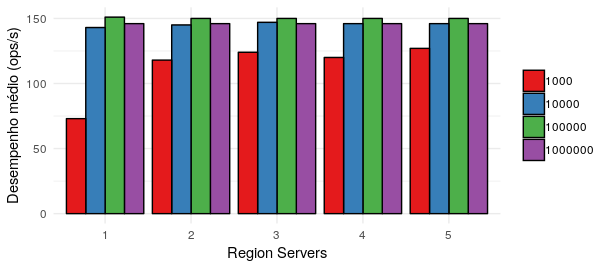
\includegraphics[width=\textwidth]{images/figura21}
        \caption{Desempenho médio.}
        \label{figura21}
    \end{subfigure}
    \begin{subfigure}[b]{0.49\textwidth}   
        \centering 
        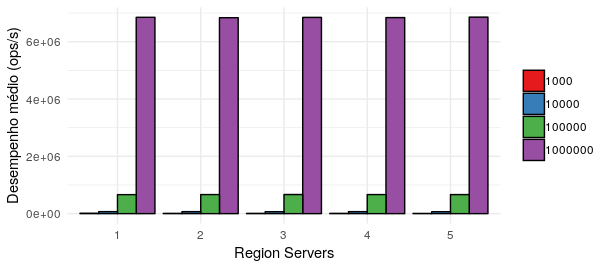
\includegraphics[width=\textwidth]{images/figura22}
        \caption{Latência.}
        \label{figura22}
    \end{subfigure}
    \caption{\emph{Workload} 100\% scan variando o tamanho do conjunto de dados e o número de region servers do cluster.}
\end{figure*}

\section{Considerações Finais}
\label{sec:finais}

Este trabalho analisou a escalabilidade horizontal de um~\emph{cluster}  Hbase, submetendo o banco de dados a um benchmarking apoiado pela ferramenta YSCB. 
Foram conduzidos testes com diferentes números de nós-escravos e tamanho do conjunto de dados.

Os resultados obtidos mostram que o escalonamento horizontal é mais evidente, considerando as~\emph{workloads} 100\%~\emph{write},~\emph{read} e~\emph{read/modify/write}, para conjuntos superiores a cem mil registros. 
Também foi identificado que o aumento do desempenho médio do~\emph{cluster}  é mais significativo no aumento de~\emph{region servers} de 1 para 2 e de 2 para 3, sendo menos expressivos a partir de 3~\emph{region servers} (inferior a 8\%).

Desta forma, a melhora no desempenho do~\emph{cluster}  Hbase, considerando o desempenho médio e a latência das operações, é diretamente proporcional ao tamanho do conjunto de dados, de modo mais evidente. 

%Por exemplo, o aumento do desempenho médio nos testes da~\emph{workload} 100\%~\emph{write} -- 1.000.000 de registros, aumentando de 1 para 5~\emph{region servers} foi de aproximadamente 47\%, enquanto para os conjuntos de tamanho 100.000, 10.000 e 1.000 registros, esse aumento foi de aproximadamente 43\%, 11\% e 5\% respectivamente.

O ganho de desempenho também varia de acordo com as operações realizadas no banco de dados. Por exemplo, o melhor aproveitamento do~\emph{cluster}  levando em conta o desempenho médio nas execuções com 5~\emph{region servers} foi alcançado pelos testes da~\emph{workload} 100\%~\emph{read}, sendo maior que os testes das~\emph{workloads} 100\%~\emph{write} e 100\%~\emph{read/modify/write} em aproximadamente 22\% e 28\% respectivamente.
Contudo, 
Os testes da~\emph{workload} 100\%~\emph{scan} mostraram que não há melhora no desempenho do~\emph{cluster}  para busca de registros, de modo independente do tamanho do conjunto de dados, devido a busca linear implementada pela ferramenta Hbase não ganhar eficiência a medida que novos nós são adicionados. 
%Exceto nos testes em que o conjunto de dados foi igual a 1.000 registros, todos testes apresentaram os mesmos resultados quanto a desempenho médio e latência. 
%Os testes em que o conjunto de dados foi igual a 1.000 teve um aumento no desempenho médio de 42\%. Isso ocorreu pois o conjunto de dados por ser pequeno, foi menos fragmentado entre os servidores escravos que os outros conjuntos.

Os trabalhos futuros podem explorar o aumento do fator de replicação, não empregado neste trabalho, ao analisar o impacto que as operações adicionais de replicação
podem causar à eficiência do~\emph{cluster} , considerando a inserção de novos nós.


\bibliographystyle{sbc}
\bibliography{sbc-template}

\end{document}
